\documentclass[border=2pt]{standalone}
\usepackage{tikz}
\usetikzlibrary{arrows.meta,positioning,calc,fit,backgrounds,shapes.geometric}
\usepackage{amsmath,amssymb}
\usepackage{times}
\definecolor{ink}{HTML}{243447}
\definecolor{cA}{HTML}{4477AA}
\definecolor{cB}{HTML}{CC6677}
\definecolor{cAu}{HTML}{44AA99}
\definecolor{cS}{HTML}{CCAA33}
\definecolor{grn}{HTML}{228833}
\definecolor{rose}{HTML}{AA3377}
\definecolor{inst}{HTML}{F2E3B3}
\tikzset{
 pap/.style={circle,draw=ink,line width=.6pt,minimum size=15pt,inner sep=0pt,font=\scriptsize\bfseries,text=white},
 aut/.style={rectangle,draw=ink,line width=.6pt,minimum size=13pt,inner sep=0pt,fill=cAu,font=\scriptsize\bfseries,text=white},
 sub/.style={diamond,draw=ink,line width=.6pt,minimum size=17pt,inner sep=0pt,fill=cS,font=\scriptsize\bfseries,text=white},
 gone/.style={draw=ink!35,fill=ink!8,text=ink!40,dashed},
 ed/.style={draw=ink,line width=.7pt},
 msg/.style={-{Stealth[length=4pt]},line width=.9pt,draw=rose},
 ptitle/.style={font=\footnotesize\bfseries,text=ink,anchor=west},
 note/.style={font=\scriptsize,text=ink,align=center},
}

\tikzset{
 est/.style={rectangle,draw=grn,fill=grn!15,line width=.5pt,minimum size=6pt,inner sep=0pt},
 fst/.style={circle,fill=rose,inner sep=1.7pt},
 tie/.style={line width=.75pt,draw=rose,{Stealth[length=3.5pt]}-{Stealth[length=3.5pt]},shorten <=1pt,shorten >=1pt},
 tieg/.style={tie,draw=grn,line width=.6pt},
 ghostedge/.style={draw=ink!35,dashed,line width=.6pt},
}
% one running-example graph; argument = name prefix
\newcommand{\running}[1]{
 \node[pap,fill=cA] (#1P1) at (0,0) {P1};
 \node[aut] (#1A7) at (1.2,0.75) {A7};
 \node[sub] (#1S3) at (1.2,-0.8) {S3};
 \node[pap,fill=cB] (#1P9) at (2.4,0) {P9};
 \node[pap,fill=cA] (#1P4) at (2.4,1.5) {P4};
 \draw[ed] (#1P1)--(#1A7) (#1A7)--(#1P9) (#1A7)--(#1P4) (#1P1)--(#1S3) (#1S3)--(#1P9);
}
\begin{document}
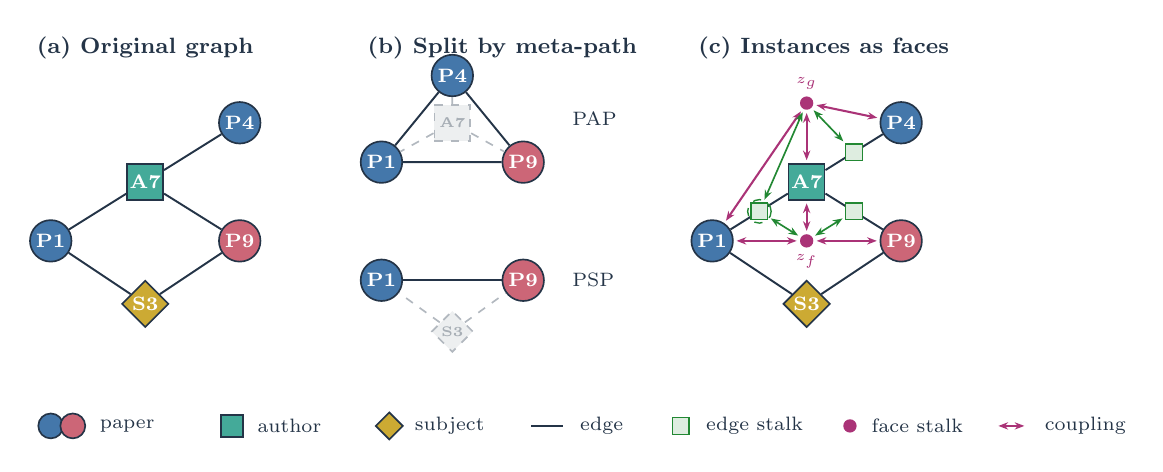
\begin{tikzpicture}
\def\TY{2.45}% common y of the panel titles
\def\XA{0}\def\XB{4.2}\def\XC{8.4}% common x of the panels
% ---------- (a)
\begin{scope}[shift={(\XA,0)}]
\node[ptitle] at (-0.3,\TY) {(a) Original graph};
\running{a}
\end{scope}
% ---------- (b)
\begin{scope}[shift={(\XB,0)}]
\node[ptitle] at (-0.3,\TY) {(b) Split by meta-path};
% PAP graph: triangle; the collapsed author sits inside, dashed
\node[pap,fill=cA] (bP1) at (0,1.0) {P1};
\node[pap,fill=cB] (bP9) at (1.8,1.0) {P9};
\node[pap,fill=cA] (bP4) at (0.9,2.1) {P4};
\node[aut,gone,minimum size=13pt,font=\tiny\bfseries] (gA) at (0.9,1.5) {A7};
\draw[ghostedge] (gA)--(bP1) (gA)--(bP9) (gA)--(bP4);
\draw[ed] (bP1)--(bP9) (bP1)--(bP4) (bP4)--(bP9);
\node[note,anchor=west] at (2.3,1.55) {PAP};
% PSP graph
\node[pap,fill=cA] (cP1) at (0,-0.5) {P1};
\node[pap,fill=cB] (cP9) at (1.8,-0.5) {P9};
\node[sub,gone,minimum size=15pt,font=\tiny\bfseries] (gS) at (0.9,-1.15) {S3};
\draw[ghostedge] (gS)--(cP1) (gS)--(cP9);
\draw[ed] (cP1)--(cP9);
\node[note,anchor=west] at (2.3,-0.5) {PSP};
\end{scope}
% ---------- (c)
\begin{scope}[shift={(\XC,0)}]
\node[ptitle] at (-0.3,\TY) {(c) Instances as faces};
\running{o}
\node[est] (s0) at ($(oP1)!0.5!(oA7)$) {};
\node[est] (s1) at ($(oA7)!0.5!(oP9)$) {};
\node[est] (s2) at ($(oA7)!0.5!(oP4)$) {};
\node[draw=grn,circle,inner sep=3pt,line width=.5pt,dashed] at (s0) {};
\node[fst] (zf) at (1.2,0.0) {};
\node[rose,font=\tiny] at (1.2,-0.26) {$z_f$};
\node[fst] (zg) at (1.2,1.75) {};
\node[rose,font=\tiny] at (1.2,2.0) {$z_g$};
\foreach \n in {oP1,oP9,oA7} \draw[tie] (zf)--(\n);
\foreach \n in {oP1,oP4,oA7} \draw[tie] (zg)--(\n);
\foreach \e in {s0,s1} \draw[tieg] (zf)--(\e);
\foreach \e in {s0,s2} \draw[tieg] (zg)--(\e);
\end{scope}
% ---------- legend, evenly spaced
\begin{scope}[shift={(0,-2.35)}]
\def\g{2.0}
\node[pap,fill=cA,minimum size=9pt] at (0,0) {}; \node[pap,fill=cB,minimum size=9pt] at (0.28,0) {}; \node[note,anchor=west] at (0.5,0) {paper};
\node[aut,minimum size=8pt] at (\g+0.3,0) {}; \node[note,anchor=west] at (\g+0.5,0) {author};
\node[sub,minimum size=10pt] at (2*\g+0.3,0) {}; \node[note,anchor=west] at (2*\g+0.5,0) {subject};
\draw[ed] (3*\g+0.1,0)--(3*\g+0.5,0); \node[note,anchor=west] at (3*\g+0.6,0) {edge};
\node[est] at (4*\g+0.0,0) {}; \node[note,anchor=west] at (4*\g+0.2,0) {edge stalk};
\node[fst] at (5*\g+0.15,0) {}; \node[note,anchor=west] at (5*\g+0.3,0) {face stalk};
\draw[tie] (6*\g+0.0,0)--(6*\g+0.4,0); \node[note,anchor=west] at (6*\g+0.5,0) {coupling};
\end{scope}
\end{tikzpicture}
\end{document}
